\documentclass[a4paper,11pt]{article}

%A Few Useful Packages
\usepackage{marvosym}
\usepackage{fontspec} 					%for loading fonts
\usepackage{xunicode,xltxtra,url,parskip} 	%other packages for formatting
\RequirePackage{color,graphicx}
\usepackage[usenames,dvipsnames]{xcolor}
\usepackage[big]{layaureo} 				%better formatting of the A4 page
% an alternative to Layaureo can be ** \usepackage{fullpage} **
\usepackage{supertabular} 				%for Grades
\usepackage{titlesec}					%custom \section
\usepackage{xeCJK}						%chinese
\usepackage{graphicx}
\usepackage{geometry}
\usepackage{wrapfig}

%\geometry{papersize={20cm,15cm}}
\geometry{top=1cm,bottom=1cm}


%Setup hyperref package, and colours for links
\usepackage{hyperref}
\definecolor{linkcolour}{rgb}{0,0.2,0.6}
\hypersetup{colorlinks,breaklinks,urlcolor=linkcolour, linkcolor=linkcolour}

%FONTS
\defaultfontfeatures{Mapping=tex-text}
%\setmainfont[SmallCapsFont = Fontin SmallCaps]{Fontin}
%%% modified for Karol Kozioł for ShareLaTeX use
\setmainfont[
SmallCapsFont = Fontin-SmallCaps.otf,
BoldFont = Fontin-Bold.otf,
ItalicFont = Fontin-Italic.otf
]
{Fontin.otf}
\setCJKmainfont[BoldFont={黑体}]{STXihei} %设置 CJK 主字体为 SimSun (宋体)

%%%

%CV Sections inspired by: 
%http://stefano.italians.nl/archives/26
\titleformat{\section}{\Large\scshape\raggedright}{}{0em}{}[\titlerule]
\titlespacing{\section}{0pt}{3pt}{3pt}
%Tweak a bit the top margin
%\addtolength{\voffset}{-1.3cm}

%Italian hyphenation for the word: ''corporations''
\hyphenation{im-pre-se}

%-------------WATERMARK TEST [**not part of a CV**]---------------
\usepackage[absolute]{textpos}

\setlength{\TPHorizModule}{30mm}
\setlength{\TPVertModule}{\TPHorizModule}
\textblockorigin{2mm}{0.65\paperheight}
\setlength{\parindent}{0pt}

%--------------------BEGIN DOCUMENT----------------------
\begin{document}

%WATERMARK TEST [**not part of a CV**]---------------
%\font\wm=''Baskerville:color=787878'' at 8pt
%\font\wmweb=''Baskerville:color=FF1493'' at 8pt
%{\wm 
%	\begin{textblock}{1}(0,0)
%		\rotatebox{-90}{\parbox{500mm}{
%			Typeset by Alessandro Plasmati with \XeTeX\  \today\ for 
%			{\wmweb \href{http://www.aleplasmati.comuv.com}{aleplasmati.comuv.com}}
%		}
%	}
%	\end{textblock}
%}

\pagestyle{empty} % non-numbered pages

\font\fb=''[cmr10]'' %for use with \LaTeX command

%--------------------TITLE-------------
\par{
		\begin{center}{\Huge 张 \textsc{政}
	}\end{center}
\begin{center}{ZHANG \textsc{ZHENG}
	}\end{center}
\par}

%--------------------SECTIONS-----------------------------------
%Section: Personal Data
\begin{wrapfigure}{r}{0.19\textwidth} %this figure will be at the right
    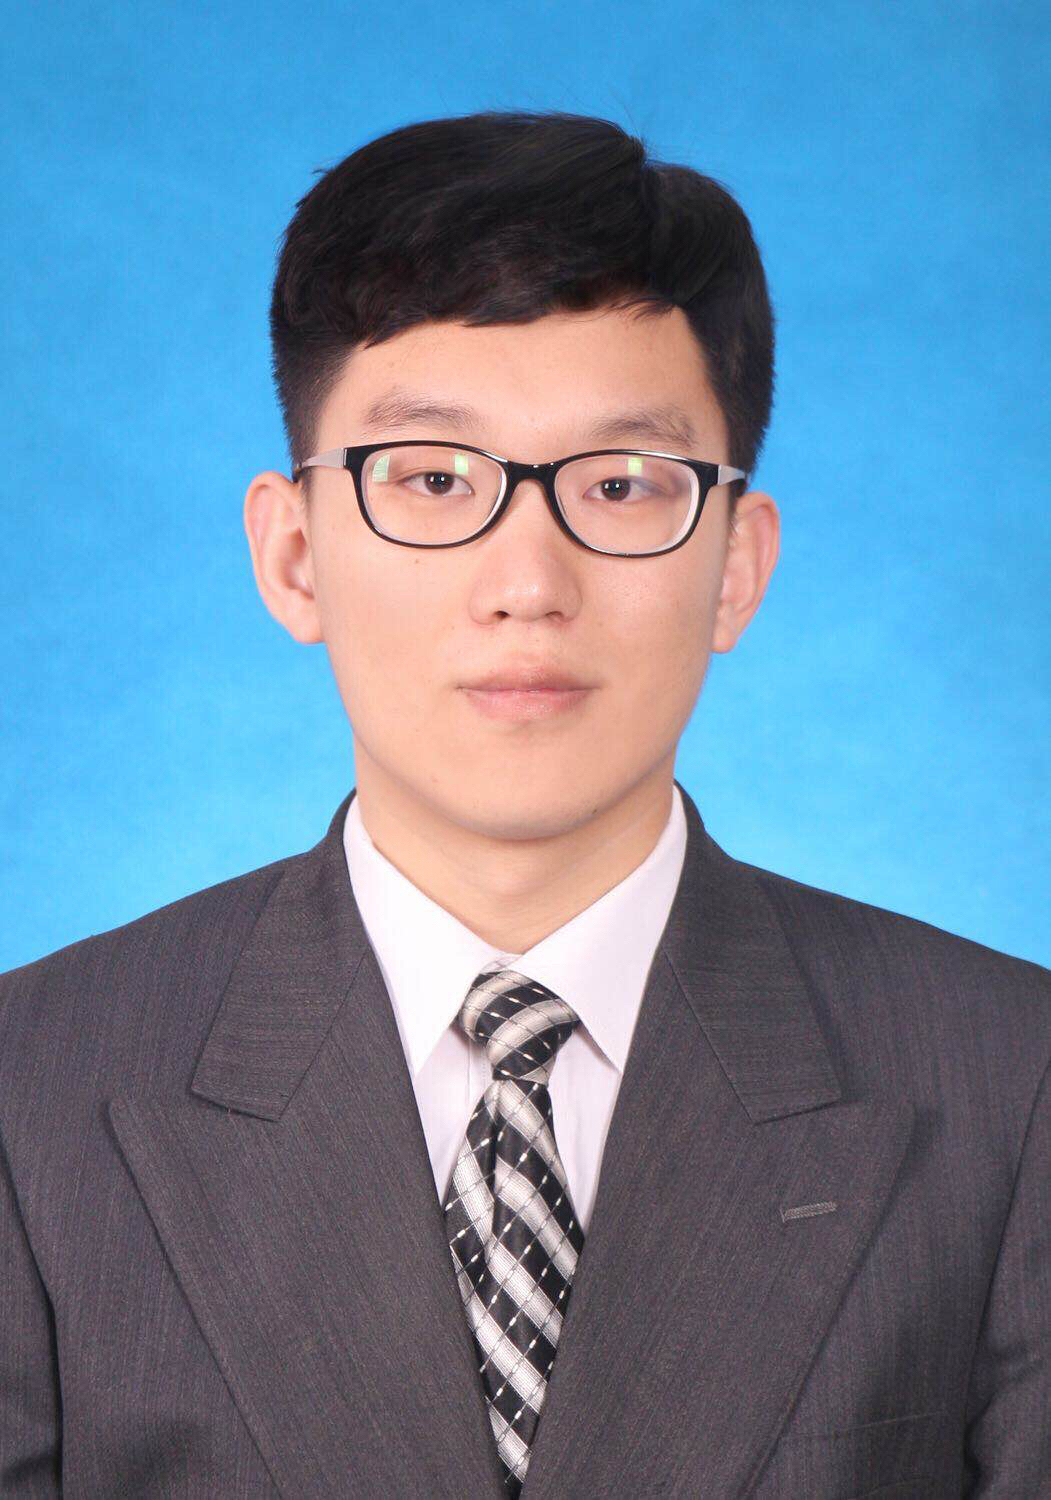
\includegraphics[width=0.19\textwidth]{pic.jpg}
\end{wrapfigure}
\section{Basic Info}
\begin{tabular}{rl}
  \textsc{Birthday:} & 1993.12.03 \\
  \textsc{Birthplace:} & Hebi, Henan province \\
  \textsc{Address:}   &  SJTU, No.800, Dongchuan Road, Minhang District\\
  \textsc{Tel:}     & 18818272991\\
  \textsc{E-mail:}     & \href{mailto:18818272991@163.com}{18818272991@163.com}\\
  \textsc{Blog:}     & \href{https://zzsean.github.io}{https://zzsean.github.io}\\
\end{tabular}



%Section: Education
\section{Education}
\begin{tabular}{rl}
\textsc{2012.9} & \bf{Bachelor, SJTU, SEIEE, IE}\\
& Academic Score Rank: Top 1\%\\
& Course: Analog Circuit, Discrete Mathematics, Data Structure, Program Design\\&\\
\textsc{2016.9} & \bf{Master, SJTU, SEIEE, IE}\\
& Course: Digital Signal Processing, Weak Signal Detection, Vision Inspection\\&\\
\textsc{2017.10} & \bf{Coursera Machine Learning.ai}\\
& Relevant principles and algorithms of traditional machine learning, such as\\
& Decision Tree, KNN, LR, SVM, and theirs derivation process and\\
& corresponding code implementation\\&\\
\textsc{2017.11} & \bf{Coursera Deep Learning.ai \& Stanford open class CS231n}\\
& Common deep neural network models such as VGG, GoogLeNet, LSTM\\
& theirs structure features and corresponding code implementation,\\ 
& Tensorflow, PyTorch, Keras and\\
& adjusting parameter and kinds of optimizers
\end{tabular}

%Section: Work Experience at the top
\section{Intern}
\begin{tabular}{r|p{11cm}}
 \textsc{2018.6 - 9} & HUAWEI, Hisi Descartes, Algorithm Engineer \\&\footnotesize{Testing the existing model and analyzing the results; Proposing the optimization scheme of related functions in the project combining the algorithms in the GPU with the computer architecture and other related knowledge; Responsible for writing scripts that automate workflows; Implementing remote distributed compilation; Familiar with the GPU architecture, understand the mainstream GPU architecture and its characteristics; Learning the use of OpenGL ES.}\\\multicolumn{2}{c}{} \\
\end{tabular}

%Section: Work Experience at the top
\section{Competition\&Project}
\begin{tabular}{r|p{11cm}}
\textsc{2018.6 - 8} & Kaggle: Google AI Open Images - Object Detection Track (top20\%)\\&\footnotesize{Image object detection and recognition and the final submitted result contains: The category name of all identified objects in each image, confidence and frame position. Training set is from Google Open Images, about 1.7 million, 600 classes. The implementation method is: Implementing YOLOv3 using Pytorch, including forward propagation, detection network and NMS, modifying the output expression to meet the competition requirements.}\\\multicolumn{2}{c}{} \\
\textsc{2018.2} & Generative Adversarial Networks(GAN)\\&\footnotesize{Implementing the game between generator and discriminator.In this project, the construction of neural network framework is completed by Tensorflow. Because the image features in the MNIST data set are relatively simple, an attempt was made to implement generator and discriminator by using different neural network structures with only full convolutional layer and convolved layer with different activation function like Leaky Relu and Relu.}\\\multicolumn{2}{c}{} \\
\end{tabular}

%Section: Work Experience at the top
\section{Competition\&Project}
\begin{tabular}{r|p{11cm}}
\textsc{2017.12} & Image Caption and Description\\{- 2018.1}&\footnotesize{The data set is from MSCOCO. The training process is divided into two steps: encoding and decoding. The neural network framework is constructed using Tensorflow. The process of encoding is to extract the features maps through CNN(such as VGG-19) and input them into the hidden layer of the sequence model RNN/LSTM; the process of decoding is to generate the text description of the image content through sequence model and word embedding training.  }\\\multicolumn{2}{c}{} \\
\textsc{2017.11-12} & Style Transfer\\&\footnotesize{The neural network framework is constructed using Tensorflow. There are two cost functions to calculate: Content loss function, calculating the SSE of the feature maps obtained by CNN(such as Squeezenet) of original and generated pics; Style loss function is similar but it uses the Gram matrix after feature extraction to compute. The pre-training Generator network can accelerate the speed of image transformation and facilitate the transformation of a large number of images of a single style. }
\end{tabular}

%Section: Work Experience at the top
\section{Research}
\begin{tabular}{r|p{11cm}}
 \textsc{2017.6 -} & Electrical Apex Locator(EAL) \\&\footnotesize{The design and improvement of EAL is the main subject of master study. It includes the circuit design, writing embedded programs and data processing, mainly involving C language and MATLAB. Machine learning is applied in an innovative way, like neural network. Through tuning parameters and network optimization, the accuracy of measurement and the robustness of measurement system are improved effectively.}\\\multicolumn{2}{c}{} \\
 \textsc{2016.1 - 6} & Active noise reduction headphone \\&\footnotesize{An active noise-cancelling headset system is built by using LMS( least mean square algorithm, verified by using offline data on MATLAB) adaptive algorithm based on Labview.}\\\multicolumn{2}{c}{} \\
\end{tabular}

%Section: Scholarships and additional info
\section{Scholarships}
\begin{tabular}{rl}
 \textsc{2014}  & SJTU Outstanding Scholarship B Class\\
& "E + H" Special Scholarship\\
\textsc{2015} & SJTU Outstanding Scholarship B Class\\
\textsc{2016} & 2016 Excellent Graduate of SJTU\\
&  SJTU First-class Academic Scholarship\\

\end{tabular}

%Section: Languages
\section{Languages}
\begin{tabular}{rl}
English: CET6, 535\\
\end{tabular}

\section{Skills}
\begin{tabular}{rl}
 Language:& Python, ~~C\&C++, ~~Java, ~~MySQL \\
 Software:& MATLAB, ~~Labview, ~~Tensorflow, ~~OpenGL, ~~{\fb \LaTeX}\setmainfont[SmallCapsFont=Fontin-SmallCaps.otf]{Fontin.otf}\\
 OS:& LINUX \\
 Other: & MS Office\\
\end{tabular}

\section{Hobbies}
Soccer~~Swimming~~Singing~~Movie


\end{document}
